\documentclass[conference,a4paper]{IEEEtran}
\usepackage[T1]{fontenc}
\usepackage{amsmath,graphicx,booktabs,url,balance}
\urlstyle{same}
\begin{document}
\title{InfluenceIQ: Offline Decision-Discussion Detection with Source-Linked Meeting Review}
\author{\IEEEauthorblockN{Anushka Chatterjee, Amitkumar Racha, Sahil Awatramani, Shriyans Sahoo}\IEEEauthorblockA{Department of Artificial Intelligence \& Machine Learning\\Symbiosis Institute of Technology, Pune\\Pune 412115, Maharashtra, India\\Anushka: anushkac2311@gmail.com; Amitkumar: rachaamitkumar@gmail.com\\Sahil: sahilawatramani@gmail.com; Shriyans: shriyanssahoo2005@gmail.com\\Faculty guide: Dr. Nivedita Mishra (nivedita.mishra@sitpune.edu.in)\\\url{https://www.sitpune.edu.in/}}}
\maketitle
\begin{abstract}Reviewing meeting recordings requires locating relevant discussion while accounting for speech recognition and speaker attribution errors. This paper presents InfluenceIQ, an offline meeting-analysis system that combines local speech processing, a supervised discussion detector and source-linked evidence review. The detector combines random-forest and logistic-regression scores computed from lexical features and neighbouring dialogue acts. Suggested passages retain their original text, speaker label and recording timestamps for human inspection. An exploratory study uses manual discussion annotations from 47 meetings, separated by project series into training, development and historical evaluation cohorts. A development-selected combination achieves 39.94\% precision, 81.18\% recall and a 53.54\% F1 score on 11,136 reference dialogue acts. Its F1 score exceeds the matched forest classifier by 1.46 percentage points, although ranking quality does not improve over every baseline. Separate speech experiments show that a larger pretrained recogniser reduces Hindi word error from 50.96\% to 28.85\% on eight fixed samples, while historical English error increases. Further classifier and continuity experiments retain negative results. The measurements support a source-traceable prototype and expose precision, annotation and generalisation limits. They do not establish complete recording-level discussion accuracy or validated participant influence.\end{abstract}
\begin{IEEEkeywords}offline meeting analysis; discussion detection; speaker diarization; evidence review; Hindi--English speech.\end{IEEEkeywords}
\section{Introduction}
Meeting recordings preserve proposals, explanations and decisions, but recovering the relevant passages requires substantial manual navigation. Automatic processing can assist this task only when users can inspect the underlying evidence. Recognition errors change the words available to an extractor, and speaker errors can assign a contribution to the wrong participant. A readable report therefore needs both an explicit evaluation target and a trace back to the recording.

The CALO Meeting Assistant integrated transcription and semantic interpretation within a broader meeting-assistant architecture \cite{ref1}. InfluenceIQ investigates a bounded engineering objective: local processing and review of passages that may belong to a decision discussion. The system uses pretrained speech components rather than introducing a speech-recognition architecture. Its learned discussion detector is a conventional supervised classifier. Local inference and evidence links are implemented properties; they do not themselves demonstrate semantic correctness or algorithmic novelty.

This study asks whether wider lexical context and a development-selected forest/linear combination improve discussion-membership detection over matched lexical classifiers, and how speech-component errors constrain the interpretation of that result. The distinction between discussion and decision is central. A passage can concern a decision without recording a final agreement. Consequently, discussion suggestions do not automatically become confirmed decisions, action assignments or participant-influence evidence.

The contributions are an implemented offline review workflow that preserves source identifiers and timestamps; a comparison of four classifier families with two lexical representations under a common split and selection rule; and an explicit account of speech errors, rejected model changes and missing downstream ground truth. The evaluation is exploratory because its historical cohort has been examined during successive development rounds. The study makes no claim of state-of-the-art performance or superiority over complete commercial meeting assistants.

\section{Related Work}
Whisper provides multilingual speech recognition from large-scale weak supervision \cite{ref2}. WhisperX addresses long-form alignment and transcription \cite{ref3}. InfluenceIQ uses faster-whisper locally; it does not implement WhisperX's complete pipeline. Diarization research includes the pyannote.audio pipeline \cite{ref4} and overlap-sensitive powerset segmentation \cite{ref5}. These works motivate reporting speaker attribution separately from transcription. The evaluated application uses its configured Sherpa-ONNX speaker backend, rather than assigning another implementation's published benchmark scores to this system.

Streaming transcription research investigates policies for committing partial output \cite{ref6}. InfluenceIQ's browser preview instead submits independent, bounded audio windows and performs complete-recording analysis after capture. Draft preview text is therefore distinct from a stable streaming transcript or live speaker-identification result.

DISPLACE evaluates multilingual speaker and language diarization \cite{ref7}, \cite{ref8}, while Vistaar examines Indian-language recognition across domains \cite{ref9}. These benchmarks motivate evaluation on natural code-switched meetings. The small Hindi and Hinglish experiments reported here cannot substitute for such a benchmark.

MeetingBank provides meeting summarization data \cite{ref10}, and ExplainMeetSum associates summaries with supporting evidence \cite{ref11}. InfluenceIQ returns extractive discussion suggestions and rule-derived candidates without generating meeting summaries. These systems and datasets address related tasks; their published scores are not interchangeable baselines for binary discussion membership. The direct quantitative comparisons in this paper use classifiers trained and scored on the same reference acts.

\section{System and Discussion Detector}
\subsection{Local Processing and Evidence Review}
Fig. 1 summarises the implemented workflow. Uploaded or recorded audio is converted to a common local waveform representation. Automatic speech recognition (ASR) produces word observations, while full-recording diarization estimates speaker activity. The application caches recognition separately from speaker attribution, allowing speaker corrections to reuse saved word observations. Correcting a displayed participant name changes presentation, whereas repairing a speaker cluster requires reviewing its acoustic assignment.

Optional presentation processing extracts slide text, tables and notes. Configured lexical or embedding similarity and available slide timing support passage-to-slide links. Missing display timestamps remain missing. Unicode-aware event rules identify candidate proposals, questions, objections, agreements, decisions and actions. Evidence and interaction links support later review. These deterministic outputs coexist with the learned detector but address different targets.

\begin{figure}[t]
\centering
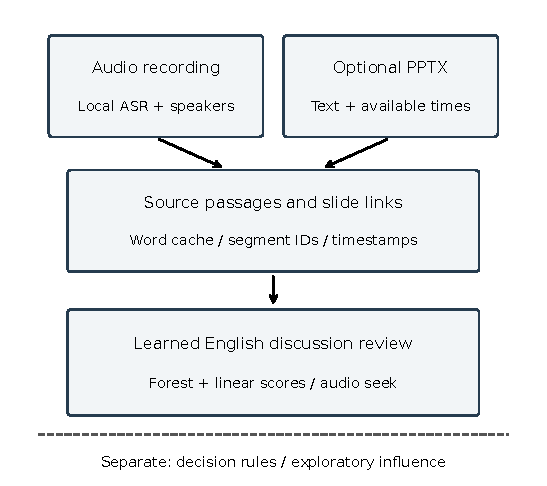
\includegraphics[width=\columnwidth]{figures/ieee_architecture.pdf}
\caption{Local processing and source-linked review. The dashed boundary separates discussion suggestions from rule-derived decisions and exploratory influence scores.}
\end{figure}
The learned stage processes final English transcript passages and stores segment identifiers, verbatim text, speaker labels, timestamps and scores. The interface provides recording seek controls, and exports retain source information. Unsupported languages and unavailable models receive explicit stage statuses. Discussion scores are ranking signals, not calibrated probabilities of correctness. Mixed-language recordings do not receive unsupported English discussion labels.

\subsection{Features and Supervised Classification}
For the research experiment, let a dialogue act contain a set of lexical word identifiers. Its binary label is one when at least half of those identifiers belong to a manually annotated decision-discussion span. Acts outside the annotated spans are treated as negatives, subject to annotation-completeness review. Dialogue-act category labels and manual decision labels are excluded from the input features.

The local representation concatenates word and character term-frequency--inverse-document-frequency features. Word features use unigrams and bigrams; character features use three- to five-character sequences. Vectorizers apply sublinear term frequency, a minimum document frequency of two and limits of 12,000 word and 20,000 character features. Vocabulary and inverse document frequency are fitted on training text. The context representation appends lexical context from up to 40 acts before and after the current act, without crossing meeting boundaries. Future context makes this an offline detector.

Four classifier families are compared: logistic regression, Complement Naive Bayes, a linear support-vector machine (SVM) and random forest. Linear classifiers use class balancing; the forest uses balanced bootstrap-sample weights. The support-vector classifier uses sigmoid calibration with three project-separated training folds. Its vocabulary is fitted on all training acts and shared across those inner folds; this limitation is disclosed rather than described as fold-specific preprocessing.

\subsection{Score Combination and Application Boundary}
The installed detector combines the previously selected context classifiers. For act i, let f(i) and l(i) denote the forest and logistic scores. The mixture is

\begin{equation}s_i=0.75f_i+0.25l_i\end{equation}
Within each meeting, scores are averaged over the current act and at most five acts on either side. If N(i) denotes this clipped neighbourhood, the predicted label is

\begin{equation}\hat y_i=\mathbf{1}\!\left[\frac{1}{|N(i)|}\sum_{j\in N(i)}s_j\geq0.357740\right]\end{equation}
The weights, smoothing radius and threshold are selected on development data. They are not adjusted for individual historical meetings. Runtime feature extraction is batched, and source text is preserved rather than rewritten. Application passages are generated by speech recognition and differ from the human dialogue acts used for training. Applying the model to these passages establishes integration; it does not transfer the oracle-input score to the application.

Participant influence remains a separate heuristic output. Independent human contribution ratings are unavailable. In the audited diagnostic recording, the proposed influence ranking equals a scaled decision-event-count baseline because the other feature families are inactive. This case cannot demonstrate an influence-model improvement.

\section{Experimental Protocol}
\subsection{Discussion Data and Separation}
The AMI corpus provides meeting recordings and manual annotations \cite{ref12}. The discussion experiment uses the 47 meetings with the relevant manual discussion spans. Table I describes the custom split. Meetings from a project series remain in one partition. The historical cohort contains three independent series, so its 12 meetings must not be treated as 12 independent participant groups. The available discussion files do not intersect the official BUT test partition; this is a custom research split.

\begin{table}[t]
\caption{Discussion-membership data split.}
\centering\footnotesize
\setlength{\tabcolsep}{2pt}
\begin{tabular}{p{0.310\columnwidth}rrr}
\toprule
Partition & Meetings & Acts & Positive acts \\
\midrule
Training & 29 & 20,339 & 5,862 \\
Development & 6 & 3,739 & 1,117 \\
Historical & 12 & 11,136 & 2,481 \\
\bottomrule
\end{tabular}
\end{table}
Reference transcripts and dialogue-act boundaries are oracle inputs. Historical labels are excluded from model fitting and threshold selection within each recorded experiment. However, the historical results have been inspected across successive experiments. All subsequent comparisons on that cohort are therefore continued exploratory development, not confirmation on a newly unseen test set. Protocols retain split membership, source hashes, frozen selections and predictions.

\subsection{Comparators, Selection and Metrics}
Each classifier family is evaluated with local features and with the additional context-40 features. The matched comparison uses three predefined model-parameter values per family, smoothing radii of 0, 5 and 15, and thresholds from 13 fixed development-score quantiles plus 0.5. Each pipeline selects its configuration by pooled development F1. The forest uses 100 trees, a minimum leaf size of two and a depth grid; the support-vector calibration uses training folds only. Equal search counts do not imply equal computational cost or exhaustive tuning.

A later combination study searches linear-mixture weights 0, 0.25, 0.5, 0.75 and 1 with the same smoothing and threshold-selection scheme. It reuses previously selected component classifiers, so its additional search budget is disclosed. Always-positive and always-negative predictors contextualise class imbalance. The initial short-context lexical study and later semantic, continuity, calibration and refit trials remain available in the supplement.

We report positive-class precision, recall and F1; average precision measures score ranking across operating thresholds. Accuracy, balanced accuracy, specificity, macro F1, the Matthews correlation coefficient and receiver-operating-characteristic area provide complementary diagnostics. No single metric is labelled overall project accuracy. A paired project-series bootstrap for the mixture-versus-forest F1 difference is descriptive because only three historical series are available.

\subsection{Speech and Diarization Pilots}
The audio pilot uses four AMI Array1-01 excerpts covering seconds 60--180. ES2002a and ES2003a form development; IS1001b and TS3007d form a locally held-out cohort. All four belong to the published BUT/pyannote training partition. Thresholds 0.5, 0.7, 0.9 and 1.1 are evaluated on development; minimum pooled diarization error selects 0.9. Scoring includes overlap, optimal speaker permutation, a 0.25-second collar and the explicit excerpt interval. References use manual speech segments, rather than the standard word-derived recipe. The resulting scores are custom pilot measurements.

Eight FLEURS Hindi recordings \cite{ref13} and eight consecutive MUCS mirror Hinglish examples \cite{ref14} form fixed recognition pilots. Source manifests preserve selection, revisions and hashes. Small, medium and large-v3-turbo models are compared where measured; Turbo is an existing pretrained recogniser \cite{ref15}, with no speech fine-tuning in this study. Inference uses a local central processing unit (CPU), 8-bit integer computation and beam size five. Automatic language detection follows the application's English/Hindi constraint. References do not supply recognition hints.

Word error is the sum of substitutions, deletions and insertions divided by reference words. Character error uses the same Unicode normalisation and excludes spaces. Normalisation applies compatibility composition, case folding and Unicode word tokenisation, without transliteration or reference correction. Rates are pooled by reference counts, not averaged across samples. Timings obtained during concurrent workloads are excluded from speed-superiority claims.

\section{Results}
\subsection{Discussion Membership}
Table II reports all eight matched classifiers and the later development-selected mixture. L denotes local word/character features, C denotes the appended context-40 representation, and AP denotes average precision. Percentages use the same 11,136 reference acts. Fig. 2 illustrates the context-model trade-off between F1 and average precision.

\begin{table}[t]
\caption{Historical discussion results; all values are percentages.}
\centering\footnotesize
\setlength{\tabcolsep}{2pt}
\begin{tabular}{p{0.330\columnwidth}rrrr}
\toprule
Model/features & Precision & Recall & F1 & AP \\
\midrule
Logistic/L & 33.29 & 91.98 & 48.89 & 50.82 \\
Naive Bayes/L & 32.67 & 91.01 & 48.08 & 48.35 \\
Linear SVM/L & 32.88 & 91.13 & 48.33 & 49.27 \\
Forest/L & 35.73 & 84.72 & 50.26 & 49.91 \\
Logistic/C & 35.61 & 87.38 & 50.60 & 56.99 \\
Naive Bayes/C & 31.60 & 92.58 & 47.12 & 57.65 \\
Linear SVM/C & 35.04 & 90.25 & 50.48 & 53.38 \\
Forest/C & 39.38 & 76.86 & 52.08 & 41.95 \\
Forest/linear/C & 39.94 & 81.18 & 53.54 & 53.40 \\
\bottomrule
\end{tabular}
\end{table}
\begin{figure}[t]
\centering
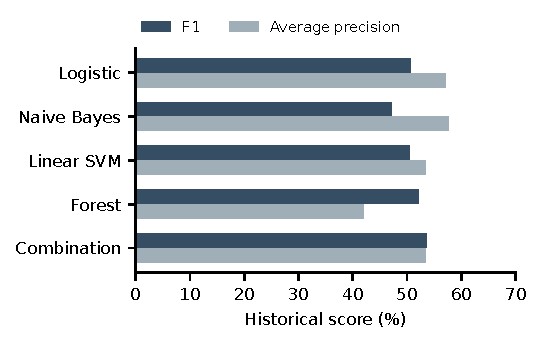
\includegraphics[width=\columnwidth]{figures/ieee_classifier_results.pdf}
\caption{Historical context-model scores. The combined model has higher F1, while other classifiers retain higher average precision.}
\end{figure}
The mixture has 59.79\% development F1 and 53.54\% historical F1, exceeding the matched forest by 1.46 percentage points. The descriptive bootstrap difference interval is \(-\)7.16 to +5.99 points; it does not establish a statistically reliable gain. Average precision increases relative to the forest but remains below the context logistic and Naive Bayes classifiers. Different metrics therefore support different model preferences.

The mixture's historical confusion counts are 5,627 true negatives, 3,028 false positives, 467 false negatives and 2,014 true positives. Accuracy is 68.62\%, balanced accuracy 73.10\%, specificity 65.01\%, macro F1 64.92\%, receiver-operating-characteristic area 80.03\% and Matthews correlation 0.3861. An always-negative predictor achieves 77.72\% accuracy with zero positive recall/F1; an always-positive predictor achieves 36.44\% F1. These controls show why class accuracy alone cannot establish useful discussion retrieval. The earlier short-context model achieved 42.35\% F1 under its separate search configuration.

Further semantic-feature and time-aware continuity searches produced no development candidate satisfying the declared non-regression requirements. A calibrated forest/Naive Bayes combination reached 60.75\% development F1 but fell to 52.93\% historical F1 and 45.91\% average precision. A fixed-configuration refit on 35 training-plus-development meetings reached 53.72\% historical F1 but reduced average precision to 48.70\%. Its larger training set prevents a matched-data superiority claim. Both replacements were rejected; their full results remain preserved.

\subsection{Multilingual Speech Recognition}
Table III lists strict pooled word and character error. E-dev and E-hist denote the two English development and historical excerpts; H and H-E denote the eight Hindi and eight Hinglish samples. Development references contain 547 words, historical English 435, Hindi 208 and Hinglish 124.

\begin{table}[t]
\caption{Fixed-sample recognition error; lower is better.}
\centering\footnotesize
\setlength{\tabcolsep}{2pt}
\begin{tabular}{p{0.310\columnwidth}rrr}
\toprule
Cohort & Model & WER (\%) & CER (\%) \\
\midrule
E-dev & small & 29.98 & 20.32 \\
E-dev & medium & 31.44 & 21.80 \\
E-dev & turbo & 28.15 & 19.76 \\
E-hist & small & 61.61 & 46.97 \\
E-hist & turbo & 63.91 & 53.52 \\
H & small & 50.96 & 20.09 \\
H & medium & 37.02 & 14.98 \\
H & turbo & 28.85 & 9.41 \\
H-E & small & 66.13 & 50.00 \\
H-E & medium & 57.26 & 52.25 \\
H-E & turbo & 57.26 & 48.31 \\
\bottomrule
\end{tabular}
\end{table}
Turbo reduces Hindi word errors from 106 to 60 and character errors from 173 to 81 on unchanged references. Its Hinglish word-error count equals medium's 71, with lower character error. Historical English instead worsens from 268 to 278 word edits. The shared application default therefore remains small, with Turbo available as an explicit local option. These results demonstrate corpus-dependent behaviour rather than a universally better recogniser. Eight correlated lecture examples cannot establish natural code-switched meeting performance.

\subsection{Speaker Calibration and Functional Evidence}
Table IV summarises the unchanged two-excerpt diarization pilot. Calibration reduces fragmentation and pooled speaker errors, while speech-region detection changes little. Matching the number of reference speakers would still be insufficient evidence of correct speaker identities.

\begin{table}[t]
\caption{Custom audio pilot before and after calibration.}
\centering\footnotesize
\setlength{\tabcolsep}{2pt}
\begin{tabular}{p{0.380\columnwidth}rr}
\toprule
Metric & Threshold 0.5 & Threshold 0.9 \\
\midrule
Diarization error (\%) & 64.08 & 40.91 \\
Jaccard error (\%) & 69.60 & 60.45 \\
Speech precision (\%) & 81.68 & 81.70 \\
Speech recall (\%) & 90.57 & 90.73 \\
Speech F1 (\%) & 85.89 & 85.98 \\
Speaker-count MAE & 8.50 & 1.50 \\
\bottomrule
\end{tabular}
\end{table}
The TS3007d reference has no supplied manual speech segment before 99.5 seconds, although the excerpt starts at 60 seconds and recognition emits introductory speech. This uncovered prefix remains included. Boundary conventions and reference coverage require an independent audio audit before interpreting the weakest scores or comparing them with official benchmark results.

The latest software regression passed 597 tests. Integration checks cover batched scoring, meeting boundaries, source preservation, missing-model behaviour, report exports and browser review. Cached real-transcript smoke checks establish execution and traceability only. They provide no independently labelled recording-level discussion accuracy, controlled speed result or physical-phone validation.

\balance
\section{Discussion and Limitations}
The experiments support a source-traceable local review system and a measurable lexical discussion classifier. They do not establish superiority of every component. A higher F1 score can coexist with worse ranking quality, and a recogniser that improves the Hindi pilot can degrade historical English. The deployment choices preserve those trade-offs rather than reporting a single combined accuracy.

Three limitations constrain the central discussion result. First, reference text and human dialogue-act boundaries differ from the longer, error-prone passages produced by recognition. Second, outside-span acts are assumed negative; incomplete discussion annotation could affect both training and measured precision. Third, only two development series and three historical series are available, and repeated historical inspection prevents treating this cohort as a fresh final test. Potential pretrained-data overlap is unknown. These factors require an independently annotated, group-separated evaluation.

Presentation alignment, final decisions, action ownership and participant influence lack task-matched independent labels. The audited influence example collapses to decision counting, and its slides lack usable timing, so existing sensitivity plots cannot establish multimodal or influence utility. A future study should activate the relevant inputs, annotate slide references and decisions independently, and compare human contribution rankings with speaking-time and decision-count baselines.

Local execution reduces dependence on remote inference but does not establish audited storage security or resolve consent obligations. Controlled cold/warm runtime, peak memory, long-recording recovery and physical-phone measurements remain absent. Concurrent pilot timings and laptop accuracy must not be assigned to Android execution. A final evaluation should separate human-transcript NLP, recognised-transcript NLP with verified speakers, and complete automatic processing to quantify error propagation.

\section{Conclusion}
InfluenceIQ implements offline meeting processing with source-linked discussion suggestions and human review. A development-selected forest/linear combination achieves 53.54\% historical discussion-membership F1 using oracle transcripts and dialogue-act boundaries. Its precision and ranking trade-offs limit the interpretation of that improvement. Separate recognition experiments show substantial Hindi pilot gains with Turbo and a historical English regression, motivating explicit model choice. Negative classifier trials, source provenance and unavailable downstream metrics remain visible. The resulting contribution is an exploratory system and comparative study. Independent recording-level annotations and controlled efficiency measurements are required before broader accuracy, influence or deployment claims.

\section*{Acknowledgment}
This B.Tech project in Artificial Intelligence \& Machine Learning was carried out by Group 12 under the guidance of Dr. Nivedita Mishra during academic year 2026--27. Student identifiers are Anushka Chatterjee (23070126015), Amitkumar Racha (24070126501), Sahil Awatramani (23070126112) and Shriyans Sahoo (23070126125).

AI assistance was used for implementation, experimental orchestration and manuscript drafting. Human authors must verify the methods, measurements and references. Funding, author contributions and applicable consent/ethics declarations remain pending author confirmation; no approval or exemption is asserted.

\begin{thebibliography}{99}
\bibitem{ref1} G. Tur et al., ``The CALO meeting assistant system,'' IEEE Trans. Audio, Speech, Lang. Process., vol. 18, no. 6, pp. 1601--1611, Aug. 2010, doi: 10.1109/TASL.2009.2038810.
\bibitem{ref2} A. Radford, J. W. Kim, T. Xu, G. Brockman, C. McLeavey, and I. Sutskever, ``Robust speech recognition via large-scale weak supervision,'' in Proc. Int. Conf. Mach. Learn., vol. 202, 2023, pp. 28492--28518. [Online]. Available: \url{https://proceedings.mlr.press/v202/radford23a.html}
\bibitem{ref3} M. Bain, J. Huh, T. Han, and A. Zisserman, ``WhisperX: Time-accurate speech transcription of long-form audio,'' in Proc. Interspeech, 2023, pp. 4489--4493, doi: 10.21437/Interspeech.2023-78.
\bibitem{ref4} H. Bredin, ``pyannote.audio 2.1 speaker diarization pipeline: Principle, benchmark, and recipe,'' in Proc. Interspeech, 2023, pp. 1983--1987, doi: 10.21437/Interspeech.2023-105.
\bibitem{ref5} A. Plaquet and H. Bredin, ``Powerset multi-class cross entropy loss for neural speaker diarization,'' in Proc. Interspeech, 2023, pp. 3222--3226, doi: 10.21437/Interspeech.2023-205.
\bibitem{ref6} D. Mach\'{a}\v{c}ek, R. Dabre, and O. Bojar, ``Turning Whisper into real-time transcription system,'' in Proc. IJCNLP--AACL: Syst. Demonstrations, 2023, pp. 17--24, doi: 10.18653/v1/2023.ijcnlp-demo.3.
\bibitem{ref7} S. Baghel et al., ``The DISPLACE challenge 2023,'' in Proc. Interspeech, 2023, pp. 3562--3566, doi: 10.21437/Interspeech.2023-2367.
\bibitem{ref8} S. B. Kalluri et al., ``The second DISPLACE challenge: DIarization of SPeaker and LAnguage in Conversational Environments,'' in Proc. Interspeech, 2024, pp. 1630--1634, doi: 10.21437/Interspeech.2024-1833.
\bibitem{ref9} K. Bhogale et al., ``Vistaar: Diverse benchmarks and training sets for Indian language ASR,'' in Proc. Interspeech, 2023, pp. 4384--4388, doi: 10.21437/Interspeech.2023-2589.
\bibitem{ref10} Y. Hu, T. Ganter, H. Deilamsalehy, F. Dernoncourt, H. Foroosh, and F. Liu, ``MeetingBank: A benchmark dataset for meeting summarization,'' in Proc. ACL, vol. 1, 2023, pp. 16409--16423, doi: 10.18653/v1/2023.acl-long.906.
\bibitem{ref11} H. Kim, M. Cho, and S.-H. Na, ``ExplainMeetSum: A dataset for explainable meeting summarization aligned with human intent,'' in Proc. ACL, vol. 1, 2023, pp. 13079--13098, doi: 10.18653/v1/2023.acl-long.731.
\bibitem{ref12} J. Carletta et al., ``The AMI meeting corpus: A pre-announcement,'' in Machine Learning for Multimodal Interaction, Lecture Notes in Computer Science, vol. 3869. Berlin, Germany: Springer, 2006, pp. 28--39, doi: 10.1007/11677482\_3.
\bibitem{ref13} A. Conneau et al., ``FLEURS: Few-shot learning evaluation of universal representations of speech,'' arXiv:2205.12446, 2022, doi: 10.48550/arXiv.2205.12446.
\bibitem{ref14} A. Diwan et al., ``MUCS 2021: Multilingual and code-switching ASR challenges for low resource Indian languages,'' in Proc. Interspeech, 2021, pp. 2446--2450, doi: 10.21437/Interspeech.2021-1339.
\bibitem{ref15} OpenAI, ``Whisper large-v3-turbo,'' model card. Accessed: Oct. 19, 2026. [Online]. Available: \url{https://huggingface.co/openai/whisper-large-v3-turbo}
\end{thebibliography}
\end{document}
